\documentclass[11pt, oneside]{article} 
\usepackage{geometry}
\geometry{letterpaper} 
\usepackage{graphicx}
	
\usepackage{amssymb}
\usepackage{amsmath}
\usepackage{parskip}
\usepackage{color}
\usepackage{hyperref}

\graphicspath{{/Users/telliott_admin/Dropbox/Tex/png/}}
% \begin{center} 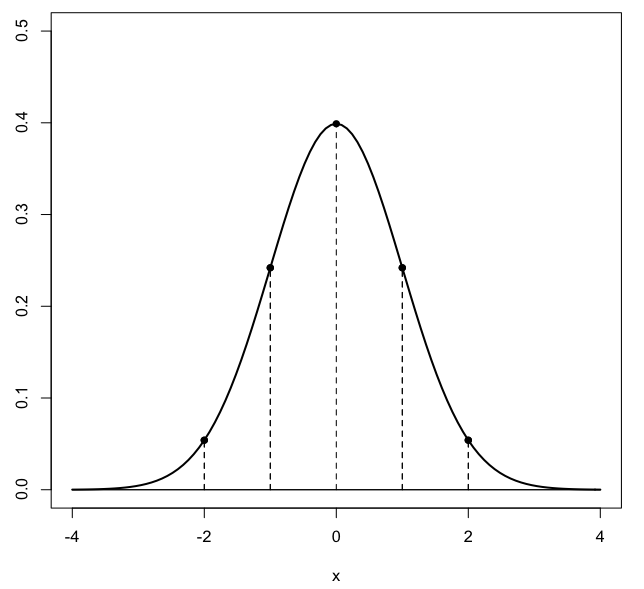
\includegraphics [scale=0.4] {gauss3.png} \end{center}

\title{Product and quotient rules}
\date{}

\begin{document}
\maketitle
\Large

The product rule says that if we have functions $u(x)$ abbreviated as $u$, and $v(x)$ as $v$ then
\[ (uv)' = u'v + uv' \]

Here is one pictorial explanation:
\begin{center} 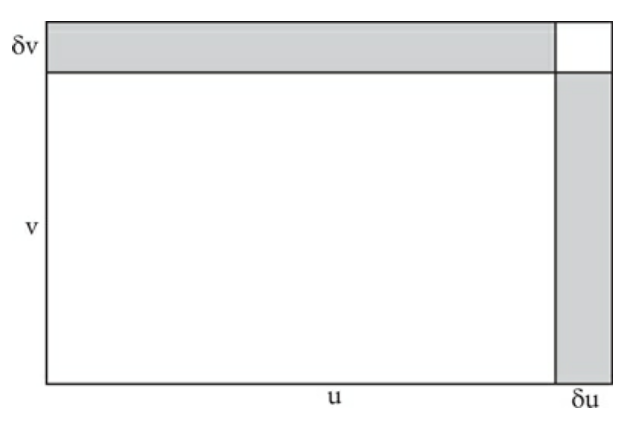
\includegraphics [scale=0.35] {product_rule2.png} \end{center}

If we have 
\[ (u + \delta u)(v + \delta v) \]
The product is 
\[ uv + u \delta v + v \delta u + \delta u \cdot \delta v \]

The difference quotient loses the first term by subtracting $uv$.  The last term is much smaller than the others because it is $\delta \times \delta$ and can be neglected.

Here is another view:
\begin{center} 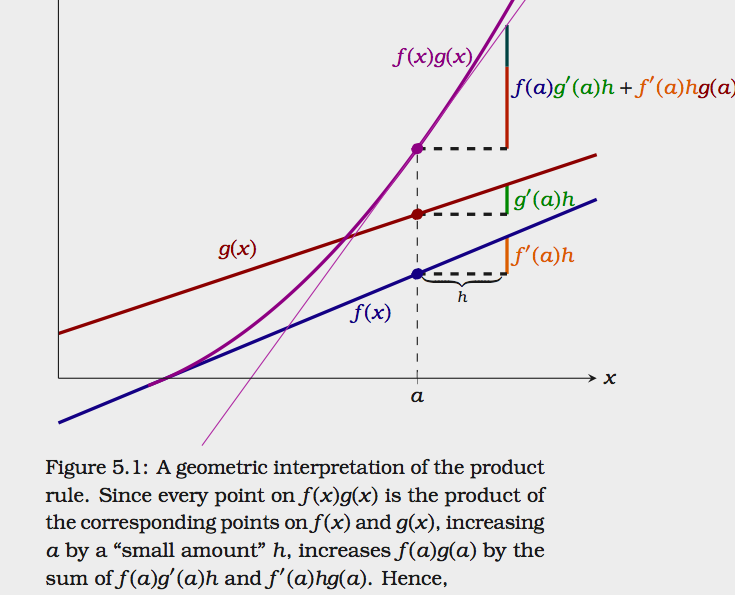
\includegraphics [scale=0.4] {product_rule.png} \end{center}

We can check this in the simplest possible ways
\[ (x)' = (1 \cdot x)' = 0 \cdot x + 1 \cdot 1 = 1 \]

\[ (x^2)' = (x \cdot x)' = 1 \cdot x + x \cdot 1 = 2x \]

\[ (x^4)' = (x^3 \cdot x)' = x^3 \cdot 1 + 3x^2 \cdot x = 4 x^3 \]
or
\[ (x^4)' = (x^2 \cdot x^2)' = x^2 \cdot 2x + 2x \cdot x^2 = 4 x^3 \]
and so on.

It is worth pointing out that one can build the general rule
\[ (x^n)' = n x^{n-1} \]
by a chain of induction based on the product rule.

\subsection*{notes}

There is a story that Leibnitz got this rule wrong at first --- the claim is that he thought the answer was $f'(x) g'(x)$.  

However, there isn't much evidence to support this.  It seems to be a slander of Leibnitz by an English supporter of Newton, as part of the wars over who invented calculus.  The supposition was shown in an unpublished notebook belonging to Liebnitz, as an example of an error.

\url{https://mathoverflow.net/questions/181422/did-leibniz-really-get-the-leibniz-rule-wrong}

The other observation is that the rule
\[ (uv)' = u'v + uv' \]
was classically recited as "this times the derivative of that, plus that times the derivative of this."  I learned it that way originally.  But if you look closely at the equation you will see that I write the reverse these days.  

The reason is that the version given above makes it easier to remember the quotient rule.

\hypertarget{quotient_rule}{}
\subsection*{inverse}
The product rule says that if we have functions $u(x)$ (abbreviated $u$), and $v(x)$ then
\[ (uv)' = u'v + uv' \]
Remember that if $u$ is not a simple function of $x$ but a compound function like $ f(g(x))$,
then $u'$ needs to take account of the inside function $g(x)$.  By the chain rule
\[ u' = f'(g(x)) \cdot g'(x) \]

As an example, when using the power rule might write
\[ (\frac{1}{v})' = (v^{-1})' = -v^{-2} = - \frac{1}{v^2} \]
and this is fine so far as it goes.  

But suppose $v$ is a compound function, like $v(t)$, the correct result is really
\[ (\frac{1}{v(t)})' = - \frac{1}{v^2} \ v'(t) \]
by the chain rule.

\subsection*{quotient rule}

Accepting this result, use it and the product rule:
\[ (u \cdot \frac{1}{v})' = u' \ \frac{1}{v} + u \ (\frac{1}{v})' \]
\[ = u' \ \frac{1}{v} + u (- \frac{1}{v^2}) v' \]
\[ = \frac{u'v - uv'}{v^2} \]

The is known as the quotient rule.

As mentioned, take care to write the product rule as $u'v + uv'$ so as to get the quotient rule by just flipping the sign of the second term and then dividing by $v^2$.

You may find yourself wondering whether you have the sign right.  Test with these two examples:

\[ \frac{d}{dx} \ \frac{x}{1} = \frac{1 \cdot 1 - x \cdot 0}{1^2} = 1 \]
\[ \frac{d}{dx} \ \frac{1}{x} = \frac{1 \cdot 0 - 1 \cdot 1}{x^2} = \frac{-1}{x^2} \]

That looks correct.  If you have the sign wrong this won't work out.

\subsection*{Strang}

Gil Strang has many wonderful takes on calculus that I haven't seen in other books.  For example:

Use the product rule here:
\[ v \cdot \frac{1}{v} = 1 \]
Take $d/dx$ of both sides.  By the product rule
\[ \frac{dv}{dx} \cdot \frac{1}{v} + v \cdot \frac{d}{dx} \ (\frac{1}{v}) = 0 \]
rearrange
\[ v \cdot \frac{d}{dx} \ (\frac{1}{v}) = - \frac{dv}{dx} \cdot \frac{1}{v}   \]
so
\[ \frac{d}{dx} \cdot (\frac{1}{v}) = -\frac{1}{v^2}  \cdot \frac{dv}{dx} \]
That's what we said!

This result extends the power rule to negative integers:
\[ \frac{d}{dx} (x^{-n}) = \frac{d}{dx} \cdot (\frac{1}{x^n}) \]
\[ \frac{d}{dx} \cdot (\frac{1}{x^n}) = - \frac{1}{(x^n)^2} \ nx^{n-1} \]
\[ = -n x^{-n-1} \]

Another one:  we establish the power rule, by induction:
\[ \frac{d}{dx} (u^{n+1}) \]
\[ = \frac{d}{dx} (u^n \cdot u) \]
\[ = (nu^{n-1} \cdot \frac{du}{dx}) \cdot u + u^n \cdot \frac{du}{dx} \]
\[ = (n+1) u^n \cdot \frac{du}{dx} \]

Since we used induction, the result applies only to integer $n$.  Later we will see proofs that extend to rational and even irrational but real numbers $n$ using implicit and logarithmic differentiation.

\subsection*{triple product}

You don't see it much, but there is a triple product rule:

\[ (uvw)' = u'vw + uv'w + uvw' \]

One might guess this is true by symmetry.  Also

\[ (uv \cdot 1)' = u'v \cdot (1) + uv' \cdot (1) + uv \cdot (1)' \]
The third term is zero, so we obtain just
\[ u'v + uv'  \]

\end{document}